\section{Major comments}

\subsection*{Reviewer comment 1}

The paper is presented as an application for ICI in combination with a
Cloudsat like configuration but it is not clear to me what geometry of
observations the authors are thinking about. They state “As mentioned above, the
same incidence angle as for the passive radiometers is assumed also for the
radar. In practice, this could be achieved by remapping the radar observations to
the lines of sights of the passive beam”. Are they thinking about a scanning
W-band radar? or at a off-nadir pointing radar? If the former is true then they
should discuss what is a realistic technological solution (and what are the
consequences in terms of sensitivity) and the authors should refer to state of
the art scanning W-band radar concepts (there is none at the moment!); if the
latter is true they should discuss what are the consequences of such a selection
(e.g. forground clutter) and they need to convince me that what we could gain
from such a configuration compensate from the loss of information introduced by
pointing in such a slanted direction. There should be a certain degree of
“realism” in what we are trying to simulate, especially if this was part of an
ESA study.

\subsubsection*{Author response:}

The reviewer raises a very relevant point with his comment. To address this, we
have changed our simulation setup to simulate perfectly co-located observations
at nadir. Realistic modeling of a space-borne viewing geometry (at least in a
variational retrieval) is currently not feasible due to the computational
complexity. We still deem this sufficient for the scope of the study, i.e.
studying the fundamental synergies between active and passive observations. In
addition to this, we follow the recommendation made in the second comment and
will pitch the application more towards air borne observations.

\subsubsection*{Changes in manuscript}

All calculations have been repeated for the assumed airborne viewing geometry
and the manuscript has been adapted accordingly.

\subsection*{Reviewer comment 2}

 “the beams of all three sensors are modeled as perfectly coincident pencil
beams”. Again this is quite an assumption. Non uniform beam filling will play a
key factor. This is one of the many simplifications (no polarization, no multiple
scattering,1D, ...) that needs to be clearly listed at the beginning of
Sect.2.2.1 (some appear only at page 27). For this reason I would actually pitch
more towards an airborne configuration where these simplification indeed can
be realistically assumed or of a radar with a radiometric mode (where you can
actually match footprints). Otherwise the (not massive) gain of having a
radar-radiometer combination that you show later on can be completely washed
out by the errors introduced to these assumptions. I imagine that you may also
have airborne data where to test how realistic your forward model is.

\subsubsection*{Author response}

%Also here we fully agree with the points raised by the reviewer. To address
%this, the second paragraph of Sect. 2.1.1 will be revised as presented in the
%previous response. Furthermore, these limitations as well as the applicability
%to airborne observations are now mentioned in the conclusions by adding the
%following lines:

As mentioned above, we will follow the reviewer's suggestion to pitch the
application of the combined retrievals more towards combined retrievals. We also
state these limitations more clear in Sect. 2.2.1 and discuss their implications
more thoroughly.

\subsubsection{Changes in manuscript}

\begin{change}[116]
\DIFdelbegin \DIFdel{A number of simplifications are applied for the generation of the synthetic
  cloud observations: Firstly, the }\DIFdelend \DIFaddbegin
\DIFadd{An airborne sensor configuration is simulated to test the retrieval. The }\DIFaddend beams
of all three sensors are \DIFdelbegin \DIFdel{modeled as
}\DIFdelend \DIFaddbegin \DIFadd{assumed to point at nadir and to be }\DIFaddend perfectly
coincident pencil beams. \DIFdelbegin \DIFdel{Secondly, a synthetic observation is
generated for each vertical profile from the model scenes by simulating a
one-dimensional, plane-parallel atmosphere, the properties of which are taken
from the corresponding model profile. It follows from these
modeling decisions
that the atmosphere is assumed to be homogeneous across the beams of the active
and passive sensors and that they all sense the same atmospheric volume. This is
certainly not }\DIFdelend \DIFaddbegin \DIFadd{Multiple scattering effects in the radar observations
as well as the effects of particle orientation are neglected. Although these
assumptions may be justified for an airborne configuration, this will not be }\DIFaddend the
case for space-borne observations \DIFdelbegin \DIFdel{and will incur a forward
modeling error that is not accounted for in this study. Since the focus of this
study are the fundamental synergies between the active and passive observations, quantifying the impact of beam width and inhomogeneity is left for future
investigation}\DIFdelend \DIFaddbegin \DIFadd{from ICI and MWI. Moreover, the incidence
angles of the beams of ICI and MWI will be around $53^\circ$ at the Earth's
surface. This further complicates the radiative transfer modeling since it
requires treating a more complex co-location geometry of the nadir-pointing
radar and the passive instruments. At off-nadir viewing angles, polarization
also needs to be taken into account, the effects of which can be several Kelvin
at the typical viewing angles of microwave imagers \mbox{%DIFAUXCMD
\citep{xie15}}\hspace{0pt}%DIFAUXCMD
.
}
\end{change}

\subsection*{Reviewer comment 3}
Fig 2: these PSDs look very weird to me. Why do they have the plateau at small
sizes? y-axis units are obviously wrong unless you are renormalizing by some mass
(but it is not explained).

\subsubsection*{Author response}

The reviewer is of course right, the units on the axis of the plots were indeed
wrong and will be corrected in the revised manuscript. Otherwise, the PSDs
correspond to the modified-gamma functions that are assumed in the
\cite{milbrandtyau05} microphysics scheme.

\subsubsection*{Changes in manuscript}

The y-units of the figure have been corrected which now looks as shown
in Fig.~\ref{fig:gem_psds}.

\begin{figure}[h!]
\centering 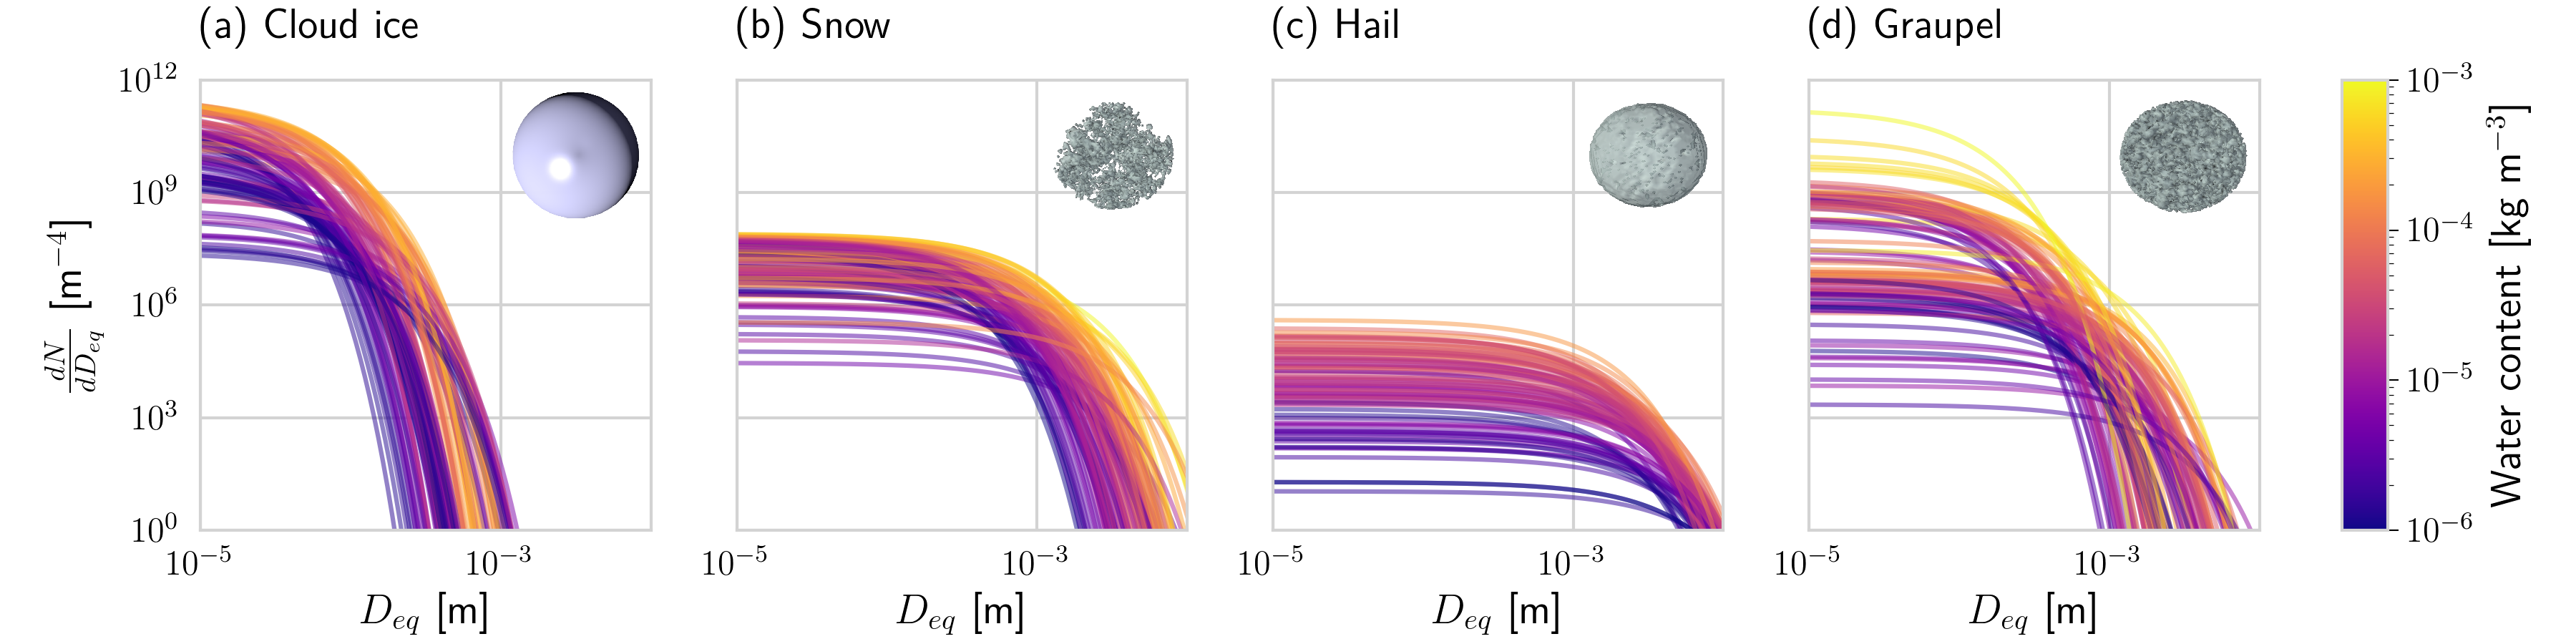
\includegraphics[width = \textwidth]{../plots/gem_psds.png}
\caption{Realizations of particle size distributions from the test scenes used
  in this study. The particle number concentration is plotted with respect to
  the volume-equivalent diameter $D_\text{eq}$. Shown are the PSDs corresponding
  to 100 randomly chosen grid points with a water content higher than
  $10^{-6}\ \unit{kg\ m^{-3}}$. Line color encodes the corresponding water
  content. Inlets display visualizations of the particle shape assumed for each
  hydrometeor species.}
\label{fig:gem_psds}
\end{figure}

\subsection*{Reviewer comment 4}

Fig 3: sorry I do not follow what is this (what is the y-axis?), and why this plot is meaningful.

\subsubsection*{Author response}

We have removed this plot from the revised version of the manuscript.

\subsection*{Reviewer comment 5}
Eq.6: Clearly with values lower than 230 K it does not make any sense (negative RH, or large than1.1???)

\subsubsection*{Author response}

We would like to thank the author to point out this inconsistency, as there are indeed two mistakes
in Eq.~6. The right equation should be
\begin{align}
\phi(t) = \begin{cases}
 0.7, & 270\ \unit{K} < t \\
 0.7 + 0.01 \cdot (t - 270), &220 < t \leq  270\ \unit{K} \\
 0.2,  & t < 220 \\
 \end{cases}.
\end{align}
This will of course be corrected in the updated version of the manuscript.

\subsubsection*{Changes in manuscript}

\begin{change}[202]
\begin{align}
\DIFdelbegin \DIFdel{\phi}\DIFdelend \DIFaddbegin \DIFadd{\text{RH}}\DIFaddend (t) = \DIFdelbegin %DIFDELCMD < \begin{cases}
%DIFDELCMD <  0.7 &, 270\ \unit{K} < t \\
%DIFDELCMD <  0.7 - 0.01 \cdot (t - 270) & ,220 < t \leq  270\ \unit{K} \\
%DIFDELCMD <  0.2 \cdot (t - 270) & ,t < 220 \\
%DIFDELCMD <  \end{cases}%%%
\DIFdelend \DIFaddbegin \begin{cases}
 0.7 &, 270\ \unit{K} < t \\
 0.7 - 0.01 \cdot (270 -t) & ,220 < t \leq  270\ \unit{K} \\
 0.2 &,t < 220 \unit{K} \\
 \end{cases}\DIFaddend .
\end{align}
\end{change}

\subsection*{Reviewer comment 6}
Line 210; this means that the vertical resolution changes with the surface temperature, really weird choice.

\subsubsection*{Author response}

We agree with the reviewer that the chosen retrieval grids may not be optimal.
We will change them to fixed-resolution grids for the revised manuscript.

\subsubsection*{Changes in manuscript}
Computations have been repeated with fix-resolution grids and the manuscript has been rewritten
accordingly.

\subsection*{Reviewer comment 7}

fIG4 : not clear to me why the scattering depression is not increasing at
higher frequencies. I would expect that the optical thickness would drastically
increase increasing frequency. Is this due to very large asymmetry parameters
then? But this is not what I do see in Fig.5 (though Fig4 is of course a very
idealized case) If this is the case then results will be very dependent on
particle habits (which may introduce additional uncertainties in the retrieval)

\subsubsection*{Author response}

It is correct that extinction increases rapidly with frequency, but the final
scattering depression depends also on other factors. One consideration is the
background absorption due to gases. A higher gas absorption decreases the effect
of scattering, and this effect generally increases with frequency. It is correct
that also the asymmetry parameter needs to be considered, which increases with
frequency. A higher asymmetry parameter gives a lower depression for a given
cloud optical depth, see Fig. 5 of \citet{eriksson15}.

It can be hard to judge the scattering depression in a figure like Fig. 5, as
the clear-sky values differ between the channels. In the version found below,
extracted scattering depressions are shown in the second panel. For high-clouds
with moderate cloud optical depth, the scattering depression increases
monotonously with frequency, while in the most dense cloud region (around lat
2.7) this is not the case for the reasons discussed above.

\begin{figure}[!hbpt]
  \centering
  \includegraphics[width=0.8\textwidth]{../plots/observations_a_3}
  \caption{Simulated brightness temperatures (Panel (a)) and cloud signal
    depressions computed for selected channels of the MWI and ICI radiometers
    for the first test scene.}
  \label{fig:depressions}
\end{figure}

\subsection*{Reviewer comment 8}
8) Line 275: not clear what you mean, in Tab.4 there are 6. 

\subsubsection*{Author response}

What was meant here is that different ice shapes are tested for the single
frozen hydrometeor species which is used in the retrieval. Tab.~4 lists the
different shape models that were investigated.

Since the section describing the selection of particle models will be rewritten,
this sentence will be reformulated to make it clearer.

\subsubsection*{Changes in manuscript}

C.f. Comments from Referee 2 - General comment 1

\subsection*{Reviewer comment 9}

9) “extends below the sensitivity limit of the passive-only observations around
10-5 kg m-3” : very sloppy sentence. Passive mi-crowave radiometer are sensitive
to integrated contents!

\subsubsection*{Author response}

As response to a comment from another reviewer the corresponding paragraph will be
rewritten and this sentence will be removed.

\subsubsection*{Changes in manuscript}

\begin{change}[310]
\DIFdel{Panel (c) shows the IWC field retrieved using the passive-only retrieval
.
Despite a certain resemblance in the overall structure between the retrieved and
reference IWCfield, the results do not reproduce }\DIFdelend \DIFaddbegin \DIFadd{results in terms of IWC. While }\DIFaddend the vertical structure of the cloud \DIFdelbegin \DIFdel{very well. It should be noted, however, that the displayed mass-density
range extends below the sensitivity limit of the passive-only observations
around $10^{-5}\ \unit{kg\ m^{-3}}$ (c.f. Fig.~4), which explains
the smeared-out appearance of the
results to some extent.}
\end{change}

%{\itshape  Panel (c) shows the IWC field retrieved using the passive-only
%  retrieval. Despite a certain resemblance in the overall structure between the
%  retrieved and reference IWC field, the results do not reproduce the vertical
%  structure of the cloud very well. It should be noted, however, that the
%  displayed mass-density range extends below the sensitivity limit of the
%  passive-only observations around $10^{-5}\ \unit{kg\ m^{-3}}$ (c.f. Fig.
%  ~\ref{fig:contours}), which explains the smeared-out appearance of the results
%  to some extent. }


\subsection*{Reviewer comment 10}

 Fig 6d: this retrieval looks really weird. Where are all the stripes coming
 from? Certainly this does not look like acloud, or? What kind of constraint
 have you imposed on the cloud top?

\subsubsection*{Author response}

It is true that the passive only retrieval does not perform well in terms of the
vertical structure of IWC. The reason for this is that the passive observations
alone do not provide much information on the vertical distribution of ice. To
correct for this, further regularization would be necessary which is not applied
here in order to keep the comparison to the other retrieval methods fair. All of
this is discussed in the discussion section of the manuscript.

\subsection*{Reviewer comment 11}

“In general, the radar-only results exhibit only very weak dependency on the
particle model, making the results for different particle shapes virtually
indistinguishable.” Again another dangerous sentence. We know (unfortunately)
that this is not true (otherwise our ice problems would be sorted). Here my guess
is that you have not properly explored the backscattering variability
(particularly looking at the different degree of riming). It is notclear to me
whether there is enough variability in your ARTS database, I guess you are more
focused at ice particles (including aggregates) but you are not considering
really rimed particles. Regions where graupel is present should be avoided from
the discussion of the radar-only retrieval for the simple reason that in those
regions attenuation correction and multiple scattering effects make the problem
very tricky. I guess that the radiometer as well is in serious trouble when
entering those areas. Again, I would not start tackling regions the observation
system is not tailored for.

\subsubsection*{Author response}

As mentioned above, we will revise the particle habits used in the retrieval,
but we expect that particle shape will continue to have a smaller impact on our
radar-only retrieval. What the results shown in scatter plot in Fig.~7 and 8
indicate is that the uncertainty which can be attributed to the particle size
distribution (PSD) is larger than that introduced by the assumed particle shape.
However, it is difficult in general to draw a clear line between particle shape
and PSD. This is especially true if particle size is described by $D\text{max}$,
and the PSD is defined accordingly. In this case, IWC of a given PSD will depend
on the particle's effective density, and e.g. degree of riming becomes critical.
Accordingly, to what extent retrieval errors are due to shape or PSD, depend
partly on definitions.

The ARTS single scattering database does include several types of rimed
particles. Two of them are the GEM Graupel and GEM Hail models which are used in
the simulation of the synthetic observations. For the retrieval, however, it is
true that we did not include rimed particles in the tested particle models but this
will be changed for the revised version of the manuscript.

Both the forward simulations and the retrieval handle attenuation consistently.
We therefore think it is worth considering even regions where graupel is present
as this allows us to assess the uncertainties caused by not having a realistic
representation of rimed particles in the retrieval.

It is certainly correct that for space-borne observations multiple scattering
needs to be considered and this will add complexity to the retrieval. Here,
however, we can avoid this extra complexity as we use simulated observations
which do not include multiple scattering.

\subsection*{Reviewer comment 12}

Fig.10 is missing!!!

\subsubsection*{Author response}

Fig. 10 was unfortunately missing from the manuscript. The figure will be included in the appendix
of the revised version together with the analysis of the second test scene.

\subsubsection*{Changes in manuscript}

C.f. Comments from Referee 1 - Minor comment 10.

\subsection*{Reviewer comment 13}
 “Since the calculation of the AVK involves the forward model Jacobian, this effectmust be related to the non-linearity of the forward model” well I would avoid such veryspeculative statements.

\subsubsection*{Author response}

Following the suggestion of the reviewer, the sentence will be removed from the manuscript.

\subsubsection*{Changes in manuscript}

The sentence has been removed from the manuscript.

\subsection*{Reviewer comment 14}
You need to be very careful how you present the results in Fig. 14. The
conclusions that I can draw is the following: a CloudSat like radar is
pro-viding much more information than the ICI+MWI radiometers when
characterizing ice particles (really the radiometer is providing some additional
water vapour information). As a result we should invest in the former and not the
latter. While I may agree with the previous statement and strongly support a
CloudSat-like radar on an operational mission my feeling is that you are
pitching your radiometer system at the wrong kind of scenes (I already see an
improvement going from the first to the second scene). I would have selected
completely different scenes (including high latitude clouds with mixed phase). It
is to me an overkill to try to retrieve D\_M of rain for these scenes from your
PMW radiometer suite of sensor. If you have any skill in warm rain you
should properly prove it

\subsubsection*{Author response}

Our interest in this study is neither arguing for one nor the other observation
system. The question that we want to address is whether combined observations
have extra value compared to separate observations. Such combined observations
could be achieved by performing joint flights with the aircraft carrying the
ISMAR sub-millimeter radiometer and another one carrying a radar, by flying a
cloud radar in constellation to Metop-SG, or by adding a sub-millimeter
radiometer to the platform carrying some future cloud radar. We consider it out
of the scope of this study to judge the cost effectiveness of either of these
solutions.

As the referee clearly favours radars, we would like to balance this by mentioning that
passive instruments have an additional strength in their much higher areal coverage. The
swath of ICI and MWI is about three orders of magnitude broader than that of CloudSat
and EarthCARE.

Although a cloud radar certainly provides more information on frozen
hydrometeors than ICI, our results clearly show that also radar observations
alone are insufficient to accurately determine the microphysical properties of
ice hydrometeors (Fig. 4, 7). The passive adds information on the microphysics
of the clouds to the radar (note the significant increase in information content
on $N_0^*$ in Fig. 14) which helps to reduce retrieval uncertainties (Fig. 11).
Although it is not clear whether these improvements carry over to space-borne
observations, our results clearly show this as a synergy between the passive and
active observations (esp. Fig. 4, 11, 14).

The cloud scenes used in the manuscript were selected with the aim of providing
a representative sampling of the type of clouds present in the two model scenes that
were available for the study. We did not want to cherry pick scenes were the
retrieval works well to provide a more realistic assessment of  the retrieval.

Rain must be handled in the retrieval due to its effect on the passive
radiances. However, we never claim that we have any skill in retrieving warm
rain and so we do not agree that we are required to prove to have it.

\subsection*{Reviewer comment 15}

 LWP and Fig.16. I have a serious problem here. The cloud I see on the right is a
 liquid cloud. So how it is possible that your radiometer is doing sobadly in
 the LWP retrieval and why the combined is so much better? I guess this must go
 back to understanding surface emissivity and integrated water vapour (maybe
 somecomments there should be made to explain what kind of surface/IWP we are
 dealingwith). You have not included radar path integrated attenuation in your
 retrieval (like istypically done in radar retrievals) but this could of course
 help in this case.

\subsubsection*{Author response}

The cloud in the right of the scene is a mixed-phase cloud. There are several
explanations for why the retrieval does not work well here: First of all, our
observations setup does not make use of the channels around $23\ \unit{GHz}$,
which are typically used for retrieving LWP. And also here the performance of
the passive-only retrieval suffers from the lack of a priori information on the
vertical position of the cloud. Since liquid water at higher altitudes has a
stronger impact on the observations, the retrieval puts too little cloud water
too high in the atmosphere because of its inability to locate it properly. This
is discussed in Sect. 4.2.3 of the manuscript.

\subsection*{Reviewer comment 16}

I do not think that for OE to work The forward model must be linear as stated at line 544.

\subsubsection*{Author response}

The OEM can of course be applied to non-linear problems but a complication that
arises is that it can get stuck in secondary minima. The sentence will be
corrected in the revised version of the manuscript.

\subsubsection*{Changes in manuscript}

The section discussing limitations of the OEM has been removed from the manuscript
since it was deemed to be of minor importance.

\subsection*{Reviewer comment 17}

17)Sect.4 and 5: a lot of waffling here (e.g. the three bullet conclusion, you
need to bemuch more quantitative and linked to what you have proved; the three
statements aresomething I could have formulated on my own without making any
simulation). Again the conclusions must be related to the cloud regime you are
considering (and cannot be valid for all!)

\subsubsection*{Author response}

One of the main advantages that we see in the combined retrieval is that it
actually works for a wide range of different cloud regimes. If the cloud regime
was known a priori, good results can probably be achieved using only a radar and
suitable a priori assumptions. In general, however, this is not the case, which
leads to the uncertainties that we currently have in the observational record
for IWP and IWC.

For the revised manuscript, we will rewrite the conclusion and parts of the discussion to make
it more concise and the point mentioned above more clear.

\subsubsection*{Changes in manuscript}

C.f. Comments from Referee 2 - Specific comment 23

\section{Minor comments}

\subsection*{Reviewer comment 1}
I would avoid the use of “ice mass density” and use “ice water content”

\subsubsection*{Author response}

The proposed changes will be adopted in the revised version of the manuscript.

\subsubsection*{Changes in manuscript}

Water content is now used consistently across the manuscript to refer to the mass
density of hydrometeors.

\subsection*{Reviewer comment 2}

Table 2:  it would be good to see footprints as well

\subsubsection*{Author response}

Since in the revised manuscript an airborne viewing geometry will be considered
the footprint sizes of MWI and ICI are not relevant anymore.

\subsection*{Reviewer comment 3}

Line 130: dBZ are the wrong units for a std of a reflectivity!

\subsubsection*{Author response}

We are unsure what the reviewer is referring to here since quantifying
uncertainty in the radar observations in dBZ seems to fairly common. This is for
example how it is handled in the DARDAR cloud \citep{delanoe10} product as well
as in the study by \citet{jiang19}.

\subsection*{Reviewer comment 4}

Line 180: “The remaining shape of each PSD is described by the shape parameters
alpha and beta, not to be confused with the parameters of themass-size
relationship shown in Tab. 1.”; very confusing. Why are you using the
same letters????

\subsubsection*{Author response}

We used the same letters to be consistent with the definition and used in
\cite{delanoe14} and \cite{cazenave18}. However, since the explicit values of
the $\alpha$ and $\beta$ parameters are probably of little interest for the
average reader, we will simply refer to \cite{cazenave18} and not name the
parameters explicitly.

\subsubsection*{Changes in manuscript}

\begin{change}[182]
\DIFdel{The retrieval computes vertical profiles of the two scaling parameters $D_m$ and
$N_0^*$ for each of the two hydrometeor species. The remaining shape of each PSD
is described by the shape parameters $\alpha$ and $\beta$, not to
be confused with the parameters of the mass-size relationship shown in
Tab.~\ref{tab:species_parameters}. The shape parameters are set to fixed, species-specific
values. This principle is illustrated in Fig.~\ref{fig:psds_retrieval}.
The plot displays the a-priori-assumed shapes of the particle size distribution
of frozen and liquid hydrometeors. The retrieved horizontal and vertical scaling
parameters }\DIFdelend , \DIFdelbegin \DIFdel{$D_m$ and $N_0^*$, are used as units for the axes of the plot so
that }\DIFdelend \DIFaddbegin \DIFadd{which scales the particle concentration, are the two retrieved
degrees of freedom of the PSD. The other two parameters describe }\DIFaddend the shape of
the \DIFdelbegin \DIFdel{PSD becomes independent of the retrieved mass density and
number concentration. For frozen hydrometeors, the values of the shape parameters $\alpha$ and $\beta$ are chosen identical to }\DIFdelend \DIFaddbegin \DIFadd{normalized PSD. The same shape parameters as in }\DIFaddend version 3 of the
DARDAR-CLOUD product \DIFdelbegin \DIFdel{\mbox{%DIFAUXCMD
\citep{cazenave18}}\hspace{0pt}%DIFAUXCMD
. For
liquid hydrometeors, the shape
parameters are chosen so that they are equivalent to }\DIFdelend \DIFaddbegin \DIFadd{\mbox{%DIFAUXCMD
\citep{cazenave20} }\hspace{0pt}%DIFAUXCMD
are chosen for frozen hydrometeors. For
rain, they are chosen to match }\DIFaddend the shape used \DIFdelbegin \DIFdel{by }\DIFdelend \DIFaddbegin \DIFadd{in }\DIFaddend the GEM model for rain drops.
\DIFdelbegin \DIFdel{All calculations involving particles size distributions
use the volume-equivalent diameter $D_\text{eq}$ as size variable.
}%DIFDELCMD < 
\end{change}

\subsection*{Reviewer comment 5}
Line 193: wrong units 

\subsubsection*{Author response}

This will be corrected in the revised version of the manuscript.

\subsubsection*{Changes in manuscript}

\begin{change}[188]
For \DIFdelbegin \DIFdel{liquid hydrometeors}\DIFdelend \DIFaddbegin \DIFadd{rain}\DIFaddend , a fixed value for $N_0^*$ of
\DIFdelbegin \DIFdel{$10^6\ \unit{m^4}$ }\DIFdelend \DIFaddbegin \DIFadd{$10^6\ \unit{m^{-4}}$ }\DIFaddend is assumed and the a priori profile for $D_m$ is
determined similarly as for frozen hydrometeors.
\end{change}

\subsection*{Reviewer comment 6}

Line 199: English

\subsubsection*{Author response}


This will be corrected in the revised version of the manuscript.

\subsubsection*{Changes in manuscript}

\begin{change}[196]
  \DIFdel{%
To further regularize the retrieval , $N_0^*$ for ice is retrieved at only 10
equally-spaced grid points between freezing layer and the tropopause. Similarly,
$D_m$ and }\DIFdelend \DIFaddbegin \DIFadd{level. The retrieval of the
  }\DIFaddend $N_0^*$ \DIFdelbegin \DIFdel{for rain are retrieved at 10
    respectively 4 points between surface and freezing layer}\DIFdelend
  \DIFaddbegin \DIFadd{parameters is further regularized by retrieving them at
    reduced vertical resolution of $2\ \unit{km}$}\DIFaddend
\end{change}

%Although this it was not exactly clear what the comment referred to, the paragraph
%has been revised and now reads as follows:
%
%{\itshape To further regularize the retrieval, $N_0^*$ for ice is retrieved at
%  only 10 equally-spaced grid points between freezing layer and the tropopause.
%  Similarly, $D_m$ and $N_0^*$ for rain are retrieved at 10 respectively 4
%  points between surface and freezing layer. This was necessary for the
%  retrieval to avoid getting stuck in spurious local minima. An approach similar
%  to this one is also taken in the GPM combined precipitation retrievals
%  \citep{grecu16}.}


\subsubsection*{Author response 7}
Line 35 page 2 (not really limited,this is a wide range!!)

\subsubsection*{Author response}

The corresponding sentence will be reformulated in the revised manuscript.

\subsubsection*{Changes in manuscript}
\begin{change}[41]
\DIFdelbegin \DIFdel{The observing frequencies that
are currently available for measuring ice from
space are limited to the
microwave, infrared and optical domain.
Infrared and
optical sensors provide sensitivity to small ice particles but cannot sense
significant parts of the ice mass of thicker clouds due to saturation of }\DIFdelend \DIFaddbegin \DIFadd{The currently most accurate information on the global distribution of ice water
content (IWC) is provided by the CloudSat radar. A main strength of these
observations is their vertical resolution, in }\DIFaddend the \DIFdelbegin \DIFdel{signal. Microwave observations , in contrast, provide sensitivity throughout the
whole atmospheric column but are insensitive to small ice particles. Although
radars and lidars generally provide greater sensitivity than their passive
counterparts, they are ultimately limited by the same principles}\DIFdelend \DIFaddbegin \DIFadd{order of 500 m.}
\end{change}

\subsection*{Reviewer comment 8}

Line 54 page 2.  maybe it is worth mentioning all the heritage coming from radar-radiometer retrievals with W-band (Ka and Ku-band) radars with PMW radiometers. 

\subsubsection*{Author response}

Following the suggestion of the reviewer, a paragraph that mentions previous work
on synergistic retrievals using radar and passive radiometers at lower microwave
frequencies will be added to the introduction.

\subsubsection*{Changes in manuscript}
C.f. Comments from Referee 2 - Minor comment 5

%{\itshape 
%... has been
%investigated \citep{evans05, jiang19}.
%
%Combined retrievals using radar and passive radiometer observations, have also
%been developed for the Tropical Rainfall Measuring Mission (TRMM,
%\citet{kummerow98, grecu04}) and the Global Precipitation Measurement (GPM,
%\cite{hou14, grecu16, munchak11}) mission. However, since the principal target
%of these missions were liquid hydrometeors, they make use of sensors at
%comparably low microwave frequencies, which provide only limited sensitivity to
%frozen hydrometeors.
%
%This work ...
%}


\subsection*{Reviewer comment 9}
Line 229: “troposphere” is too generic Line


\subsubsection*{Author response}

The use of the word {\itshape troposphere} and should have been {\itshape tropopause}.
This will be corrected in the revised version of the manuscript.

\subsubsection*{Changes in manuscript}

The section has been rewritten

\begin{change}[246]
\DIFaddbegin \DIFadd{Fig.~\ref{fig:particle_properties} provides an overview of the bulk mass
backscattering efficiencies and mass attenuation coefficients of the selected
particles computed for three different values of the }\DIFaddend $N_0^*$ \DIFdelbegin \DIFdel{is retrieved
at three equally spaced grid points between freezing layer and troposphere, while
$D_m$ is retrieved at five. For liquid hydormeteors, the retrieval grids for
$N_0^*$ and $D_m$ are reduced to two equally spaced points between surface and freezing layer. Relative humidity is retrieved at a vertical resolution of $2\ \unit{km}$}\DIFdelend \DIFaddbegin \DIFadd{parameter of the
PSD. Mass backscattering efficiency and attenuation coefficient are defined as
the ratio of the corresponding cross-section $\sigma$ and the bulk water
content:}
\end{change}


%The figure caption will be revised and now reads:
%
%{\itshape Simulated observations of a homogeneous, $5\ \unit{km}$ thick cloud
%  layer with varying water content $m$ and mass-weighted mean diameter $D_m$.
%  The panels display the maximum radar reflectivity in dBZ overlaid onto the
%  cloud signal measured by selected radiometer channels of the MWI (first row)
%  and ICI radiometers (second row).}

\subsubsection*{Author response 11}
250: rho is not defined

\subsection*{Reviewer comment}

$\rho$ will be defined in the revised version of the manuscript.

\subsubsection*{Changes in manuscript}

\begin{change}[276]
\DIFadd{Figure~\ref{fig:contours} displays }\DIFaddend the contours of \DIFdelbegin \DIFdel{the
passive cloudsignal are the isolines of the maximum radar reflectivity returned
from the cloud}\DIFdelend \DIFaddbegin \DIFadd{$\Delta T_B$ and
$\text{dBZ}_\text{max}$ with respect to $D_m$ and the cloud's water content,
which is proportional to $N_0^*$:
}\begin{align}
\DIFadd{\text{WC} = \frac{\pi \rho}{4 ^ 4}N_0^* D_m^4,
}\end{align}
\DIFadd{with $\rho$ the density of ice}\DIFaddend .
\end{change}

\subsection*{Reviewer comment 12}
Line 4: 272.5????

\subsubsection*{Author response}
This mistake will be corrected in the revised version of the manuscript.

\subsubsection*{Changes in manuscript}

\begin{change}[186]
\begin{align}
N_0^* &= \exp \left ( -0.076586 \cdot (T - \DIFdelbegin \DIFdel{272.5}\DIFdelend \DIFaddbegin \DIFadd{273.15}\DIFaddend ) + 17.948 \right ),
\end{align}
\end{change}

\subsection*{Reviewer comment 10}
Fig 4 caption: you need to include how thick is the layer.

\subsubsection*{Author response}
This will be included in the revised version of the manuscript.

\subsubsection*{Change in manuscript}

This has been changed in the revised manuscript and the figure and
caption now looks as is shown in Fig.~\ref{fig:contours}.

\bibliographystyle{copernicus}
\bibliography{references}

\end{document}
